\section{Door and cabinet recognition using Convolutional Neural Nets and real-time method fusion for handle detection and grasping \cite{7942676}}
In \cite{7942676} the authors present a method to recognize doors and cabinets. The main purpose is to capture useful features to manipulate these doors with a robotic arm. To do this, the module presented in this work has to identify the doors' handles and their characteristics. The authors presents also a robotic system to perform the physical manipulation (which is the action of open or close a door), but we only focus on the detection part. The approach proposed in this work is hybrid: it combines the potential of deep learning with the more classical feature-based algorithms. 

\begin{figure}[h!]
	\centering
	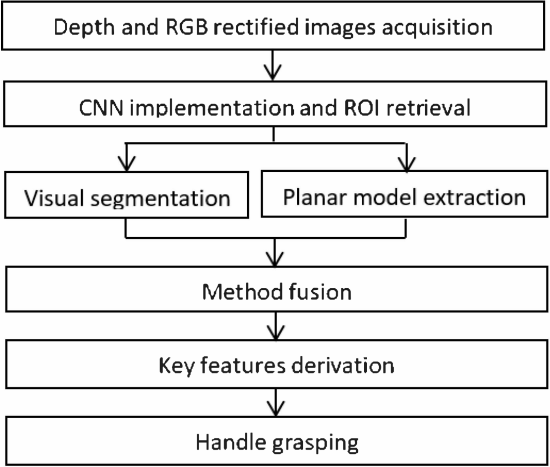
\includegraphics[width=0.4\linewidth]{images/method_overview.png}
	\caption{Pipeline of the proposed approach. It empathize the method's split after CNN.}
\end{figure}

First, the robot acquires both the depth and RGB images in order to take advantage of the combination of color and depth information. Then, the module uses a CNN (Convolutional Neural Network) which generates a ROI (region of interest), a bounding box around doors and cabinets. This technique reduces the computational time and the false-positive rates in later stages. After that, the system estimates the handle's point cloud inside the ROI using two different methods: the first one, which uses the color information, performs a visual segmentation of the ROI. Its goal is to create a clear differentiation between
the door plane and handle, under the assumption that the door's surface has a clear
color contrast with its handle. The second approach extracts the point cloud from the depth image and performs a point cloud segmentation to identify different planes inside the ROI. These two methods are combined to detect and delete the false positives generated by each of them. Finally, the handle's point cloud is identified. This article is particularly useful for our purpose because the methods proposed uses deep learning to identify a ROI and then combines effectively two different techniques (color and depth segmentation) to search for particularly useful features (the handles). Besides, this article exposes the CNN structure and pays attention to the system's efficiency. This method works well with ranges up to 1.5 meters from the door, but its performance gradually gets worse the more the distance from the target grows.

\newpage

\section{An Automated 3D Scanning Algorithm using Depth
	Cameras for Door Detection \cite{7380814}}

The work presented in \cite{7380814} exposes a method to recognize doors and their status (opened, semi-opened) using only depth data acquired by a Microsoft Kinect. The author assumes that the Kinect camera is always perpendicular to the door plane and the dimension of the door dimensions are about 2.0 x 0.9 meters. 

\begin{figure}[h!]
	\centering
	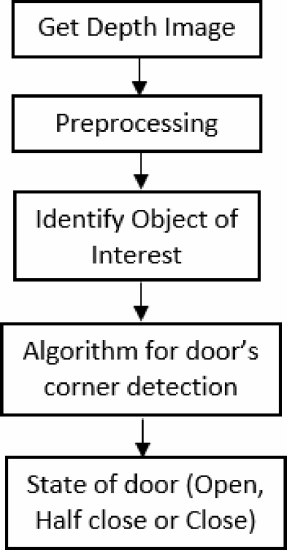
\includegraphics[width=0.20\linewidth]{images/method_kinect_only_depth.png}
	\caption{Step by step procedure to detect doors. This picture is important because it resumes the algorithm proposed in \cite{7380814}}
\end{figure}

After the depth image is taken, the object of interest is identified: the largest black color portion. This object is divided into four parts in order to identify the four corners and determine the door dimensions. The ratio calculated using the door's width and height is useful information to identify a door and find its status (open, half-open or close). The main issue about this article is that closed doors can not be detected, but those semi-opened and fully opened are successfully recognized, both from inside and outside the room. The study shows that the optimal Kinect range is around 3.3 meters.

\newpage

\section{Real-Time 3D Door Detection and Classification on a Low-Power Device \cite{9096155}}

In \cite{9096155} the authors present two methods to recognize doors and their status (open, semi-open, and closed): the first one uses both 3D and RGB data (\textbf{Method A}) while the latter uses only 3D information (\textbf{Method B}). These approaches work in low-powered systems such as the single-board computers Nvidia
Jetson Nano or the Raspberry Pi. The main contributions of this paper are a labeled dataset with RGB and depth images of closed, open, and semi-open doors and a dataset for semantic segmentation algorithms with annotated doors and door frames. The \textbf{Method A} uses a segmentation method to produce a bounding box around a ``door" in an RGB frame. Next, the depth image is cropped according to this bounding box and converted to a grayscale point cloud. Finally,  the 3D object classification PointNet is used to infer the door status (open, semi-open, and closed).

\begin{figure}[h!]
	\centering
	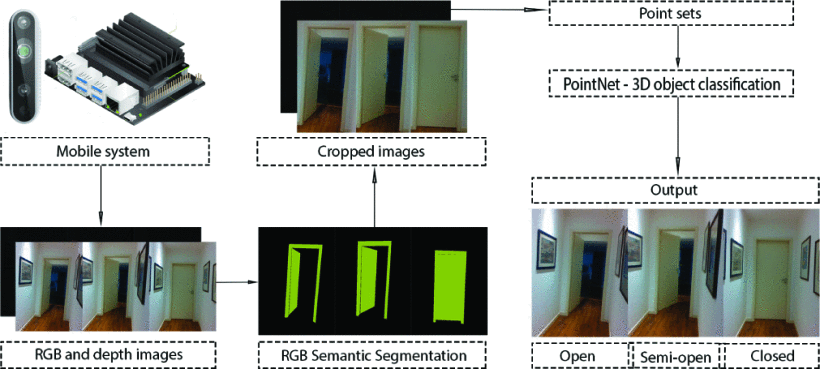
\includegraphics[width=0.48\linewidth]{images/rgb_segmentation_depth.png}
	\caption{Algorithm of \textbf{Method A}, which produces a 2D semantic segmentation and then a 3D object classification.}
\end{figure}

The \textbf{Method B} is similar to the previous one, but it uses only 3D information. It uses PointNet to classify the depth image and predict the doors' status. Unlike \textbf{Method A}, the depth image is not cropped according to a bounding box, but the number of points used as input by PointNet is the same. 

\begin{figure}[h!]
	\centering
	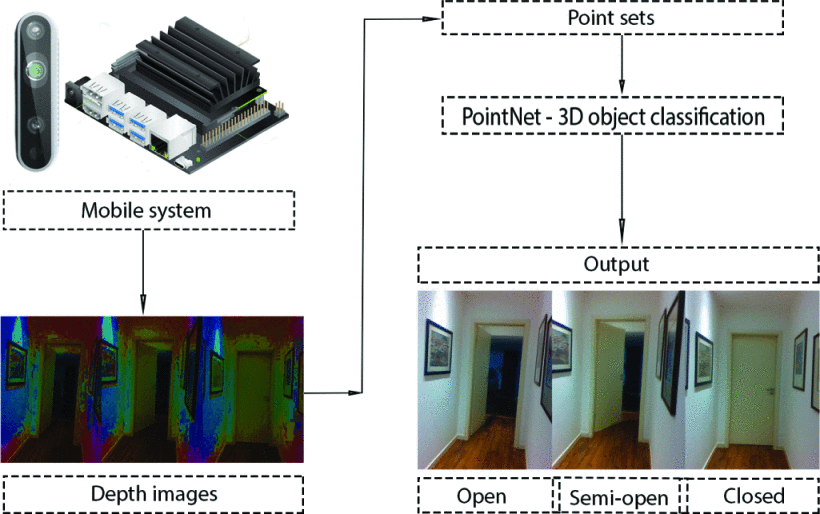
\includegraphics[width=0.48\linewidth]{images/depth_classification.png}
	\caption{Algorithm of \textbf{Method B}, which performs only 3D object classification.}
\end{figure}

This work can be useful to understand the differences between methods that use different data and provides two datasets for 3D point cloud classification and image segmentation. Despite this, this article does not focus on recognizing doors, but on determining their status.

\newpage 

\section{Door Detection in 3D Colored Laser Scans for Autonomous Indoor Navigation \cite{7743677}}

The method proposed in \cite{7743677} performs detection of open and closed doors using RGB and depth information. In particular, it presents a robust and advanced technique to successfully use and integrates color and depth information to recognize doors. First of all, this method produces a 3D simplified model of a room, composed of voxels of size 20x20x20 cm. Each voxel can be occupied or non-occupied. In this discretized space, the method detects ceilings, walls, and floors assigning a label to each voxel. The detection of open doors is focused on wall areas that present openings. To localize wall openings with precision, the authors consider not only the voxels but also the set $S$ of all the
scanned points associated with them. The first stage consists of extracting a set of candidate rectangles. To do this, the authors extract the horizontal and vertical lines in the
image with a lateral histogram technique and consider all
rectangles formed by the intersections of pairs of vertical lines
with pairs of horizontal lines. Then, the voxels' centroids are clustered by means of a region growing
algorithm. Next, the rectangles and the centroids are aligned and only the rectangles containing the highest number of centroids belonging to the same cluster are chosen as door candidates.

\begin{figure}[h!]
	\centering
	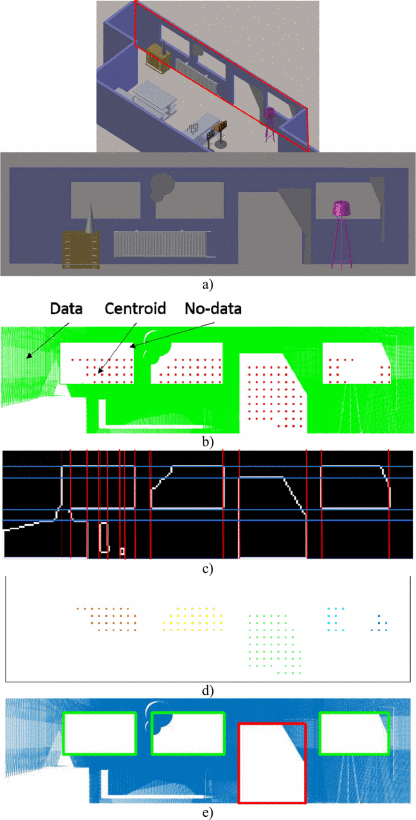
\includegraphics[width=0.30\linewidth]{images/voxel_open_doors.png}
	\caption{a) Structural element in a 3D scene with occlusion. b) Image with
		labels data, centroid and no-data. c) Vertical and horizontal lines detected in
		the image. d) Clusters of centroids in different colours. e) Openings (door and
		windows) detected. This picture visually explains all the steps to recognize an open door using only depth data.}
\end{figure}

To recognize closed doors, only 3D data are insufficient. To do this, the proposed method creates an RGB-D orthoimage of the wall where each pixel has an RGB color and the orthogonal distance to the wall plane and performs a particular segmentation technique using this image. First, small square patches (5×5 pixels) are sampled and those that are not coherent in both color and depth domain are discarded (figure 5b). Now, these patches are clustered. Finally, the method identifies the set of pixels associated with each cluster considering all the four pixel components (RGB-D). The wall area is selected as the cluster that contains the largest number of pixels located at the border of the image. 

\begin{figure}[h!]
	\centering
	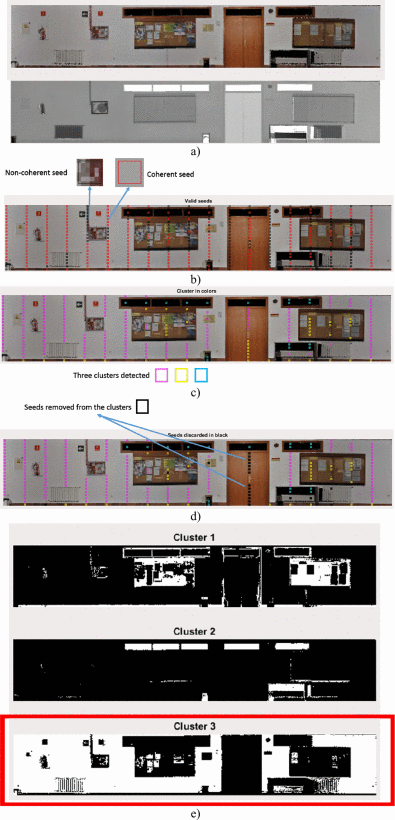
\includegraphics[width=0.25\linewidth]{images/open_doors_RGBD.png}
	\caption{Wall’s area detection. a) RGB image and depth image b) Searching
		valid small square patches (they are called seeds in the figure). c) Seed
		clusters. d) Removing inconsistent seeds from clusters. e) Segments and wall
		area identification (marked in red). This figure contains the various steps to find the wall's surface and segment its area according to color and depth information.}
\end{figure}

Then, the authors' proposal consists of elaborating separately the components of color and depth and reassembling the results at the end. This process produces a new image where the white pixels represent discontinuities in the color-depth space. 

\begin{figure}[h!]
	\centering
	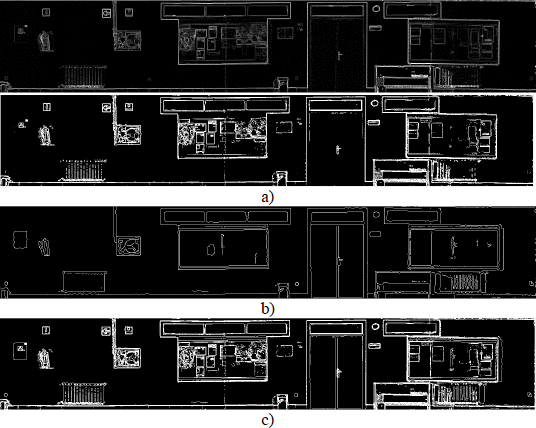
\includegraphics[width=0.25\linewidth]{images/both_rgb_depth.png}
	\caption{Generating the combined discontinuity image, combining the separate analysis of the RGB and depth data.}
\end{figure}

\newpage

\section{Door detection in 3D coloured point clouds of indoor environments \cite{QUINTANA2018146}}

The work presented in \cite{QUINTANA2018146} exposes an original approach that detects open, semi-open, and closed doors in 3D laser scanned data of indoor environments. The computation starts when the scanning of a room has been completed. The output of
this scanning is composed of a dense 3D colored point cloud, a labeled voxel model with associated 3D points from the point cloud and a 3D boundary model of the room composed of planar rectangular patches (and their associated voxels) representing the
walls, ceilings, and floors. The process to create the 3D voxel model and its labeling is explained in \cite{QUINTANA2016643}. Each voxel is labeled as either: 
\begin{itemize}
\item Occupied: The voxel contains at least one scanned point.
\item Occluded: The voxel does not contain any point and was not visible
from any of the scanning locations used to scan the room.
\item Opening: The voxel does not contain any point, despite being visible
from at least one scanning location.
\item Clutter: The voxel contains at least one scanned point but is associated with furnishings or other elements not related to the building structure.
\end{itemize}

\begin{figure}[h!]
	\centering
	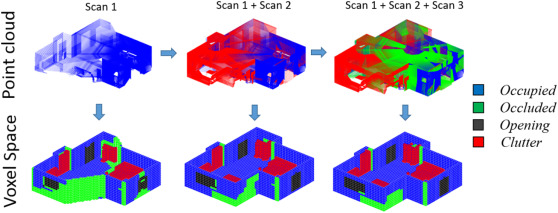
\includegraphics[width=0.80\linewidth]{images/3Dvoxel.jpg}
	\caption{Illustration of the process used to construct the
		3D voxel space and labels. This figure clearly explains how 3D data are organized.}
\end{figure}

The proposed algorithm for door detection uses as input a 4D orthoimage, one for each wall, in which each pixel has color (RGB) and depth information. Each of them is created merging all 4D orthoimages of the same wall captured from different points of view. To do this, a weighted mean color merging is proposed that considers the expected value of
the color data from each scanning location and the presence of specular highlights. The photos are collected by the camera using flash, to provide a more consistent scene's illumination. However, the use of the flash may result in specular highlights, which  must be robustly detected and corrected to ensure a correct door classification in future steps. For its detection, the following four-step algorithm is proposed:
\begin{itemize}
	\item The region of interest are located in the wall surfaces.
	\item The specular highlight region candidates are found using a quantized intensity image with 11 grey levels.
	\item The region detection is performed analyzing the intensity profile in each direction and, if any of them fits a 2D Gaussian
	function, the entire region is recognized as a specular highlight region.
	\item Each region is extended in order to be removed in future. 
\end{itemize}

\begin{figure}[h!]
	\centering
	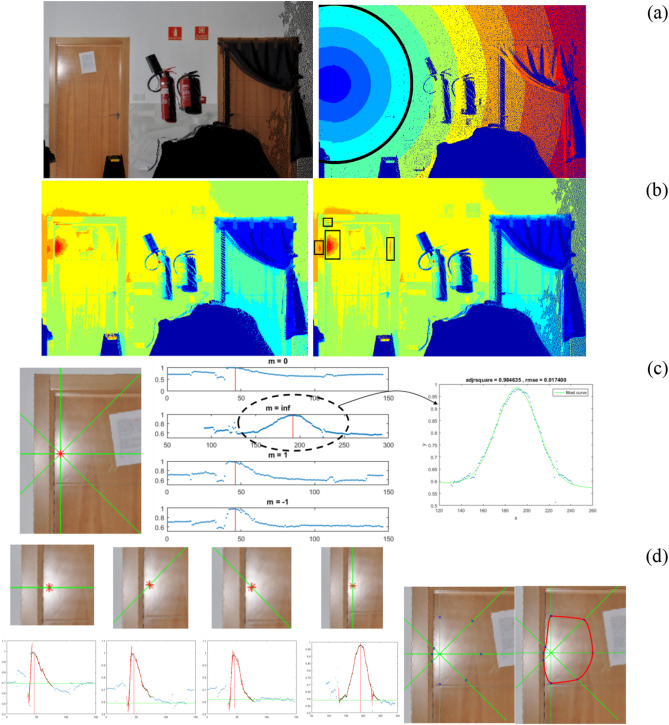
\includegraphics[width=0.78\linewidth]{images/specularregion.jpg}
	\caption{Detection of specular highlight regions in the wall. This figure exposes a robust method to detect the specular highlight regions which can be used independently regardless of the use of the flash.}
\end{figure}

The specular highlights correction is now preformed: all color information of the pixels contained in the highlight regions are discarded and refill the region using the inpainting technique reported in \cite{1467533}.
Now, the data required by the proposed method are successfully obtained and processed. The next step is to detect the door openings. First of all, the walls' trinary orthoimage is generated, in which each pixel is labeled according to the voxel labels. Then, the candidate rectangles are extracted using the intersections between pairs of vertical and horizontal lines found with a lateral histogram algorithm. Now the centroids are clustered and the
best candidate rectangles are selected as the ones with the smallest area that contains the largest number of centroids. Finally, the rectangles with their lower
side at the level of the floor are recognized as door openings.

\begin{figure}[h!]
	\centering
	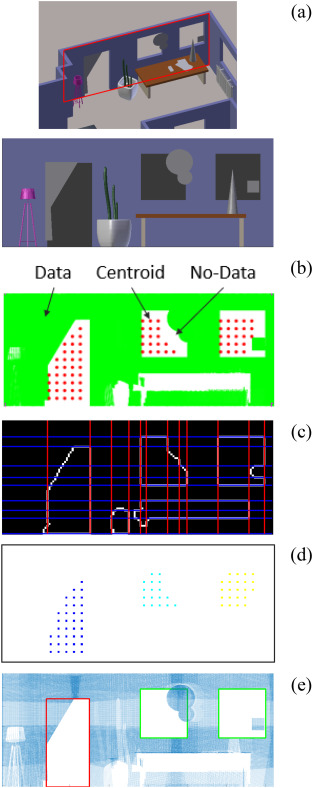
\includegraphics[width=0.3\linewidth]{images/dooropening.jpg}
	\caption{Detection of openings inside doors. This figure visually explains a robust method to recognize open doors using only depth data.}
\end{figure}

To recognize doors, the authors have developed a 4D (color + depth) approach that is able to deal with cases in which either the wall or the door does not have entirely uniform colors. The algorithm for detecting doors is divided into two steps, wall area detection and door detection. The wall detection phase works as follows:
\begin{itemize}
	\item The 4D orthoimage of a wall is divided into small patches. Those who has the standard deviation of the distribution of the RGB-D pixel values, in any of the four components, higher than a threshold, are discarded. 
	\item The remaining coherent patches are clustered.
	\item The wall area is recognized as the cluster that contains the largest number of pixels located on the left, right and top borders of the image.
\end{itemize}

\begin{figure}[h!]
	\centering
	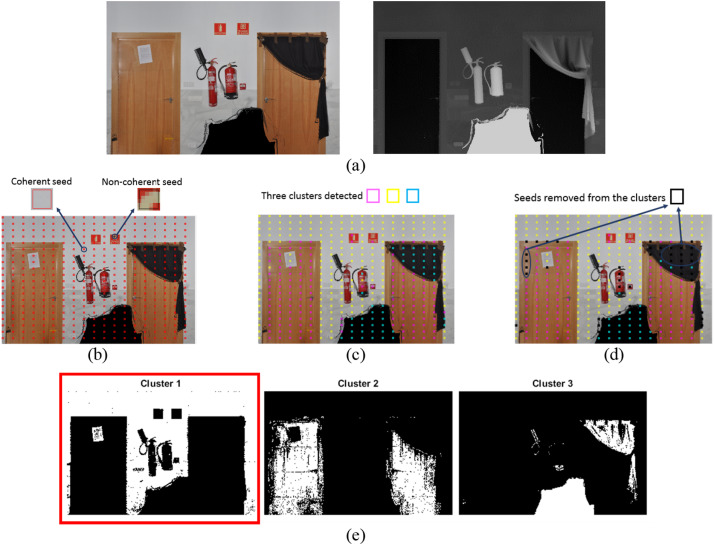
\includegraphics[width=0.8\linewidth]{images/wallrec.jpg}
	\caption{Wall area detection. The red rectangle highlights the wall surface. This figure is important because it describes a robust algorithm to detect a wall surface using color and depth information.}
\end{figure}

\newpage

The algorithm to detect doors processes the color and depth components of the orthoimage separately the results are finally recombined to produce black with the edges in white. The method is explained in the following figure.

\begin{figure}[h!]
	\centering
	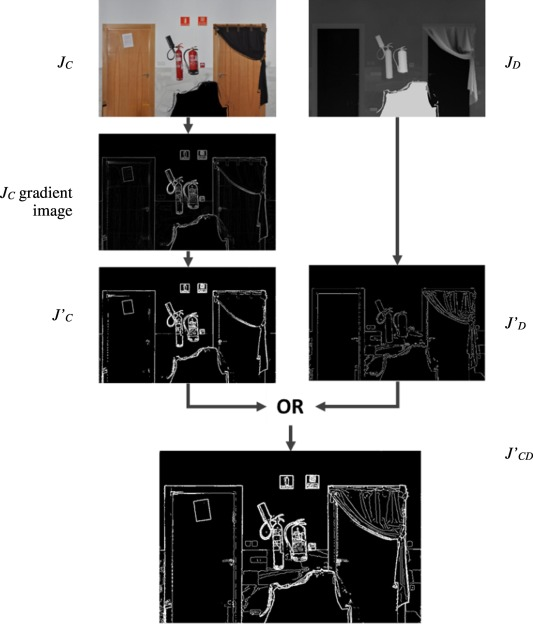
\includegraphics[width=0.6\linewidth]{images/rgbd_edges.jpg}
	\caption{Generating the combined discontinuity image. This is a robust methods to recognize edges using both color and depth information.}
\end{figure}

Now, the doors are detected by finding all the possible rectangles and the real doors are discriminated by selecting the rectangles that respect a geometric model.

\begin{figure}[h!]
	\centering
	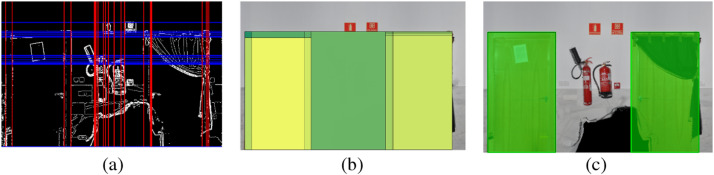
\includegraphics[width=0.9\linewidth]{images/door_edges_det.jpg}
	\caption{Door detection example.}
\end{figure}

\newpage

The final step is to determine the door opening angle. It is obtained
by taking a horizontal half-height splice of the door data and finding the
line that best fits the points of the door leaf. The figure below shows a visual example.

\begin{figure}[h!]
	\centering
	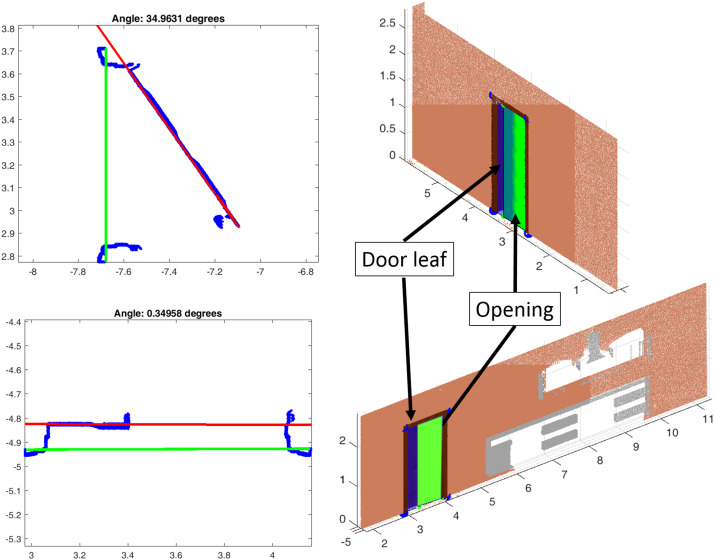
\includegraphics[width=0.7\linewidth]{images/opening_angles.jpg}
	\caption{Calculation of opening angles. On the left, the red and green lines represent the wall plane and the door leaf. This is a great approach to find the opening angle using the information calculated in the previous steps.}
\end{figure}

The approach proposed in this article is robust and handle occlusions and specular highlights. However, this method does not work in real-time and it is very computationally hard. 

\newpage

\section{Door recognition and deep learning algorithm for visual based robot navigation \cite{7090595}}
In \cite{7090595} the authors present a method to detect doors using deep learning. In particular, the proposed method uses CNN to detect doors in the environment. 

\begin{figure}[h!]
	\centering
	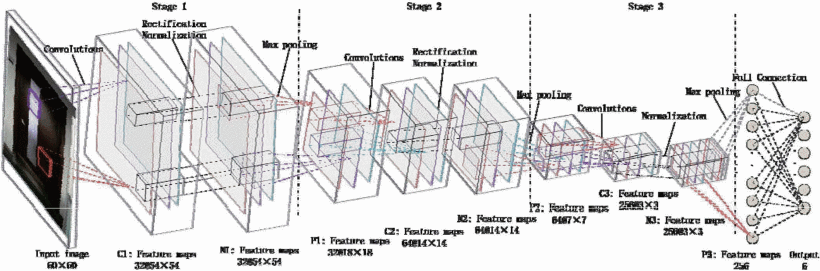
\includegraphics[width=0.9\linewidth]{images/CNN_doors.png}
	\caption{A visual representation of the proposed CNN.}
\end{figure}

The training set consists of door images taken with different angles and lighting. It has 20500 pictures (60 x 60 pixels), 2500 are positive samples while and 18000 are negatives. As explained in \cite{443235674}, the images are pre-processed to increase the network performance. The steps are: 1) to split the color images into RGB three channels and resize them to 3600 x 3 pixels; 2) to subtract the mean value and divide by the image standard deviation; 3) to apply normalization. This article details how to set up CNN. It obtains good results in the recognition of negative samples but the error ratio obtained with the positive ones is 26.5 \%.
Another negative aspect is that the article does not implement the method in a real robot in order to evaluate the CNN performance in low-power systems.

\newpage

\section{3D Modeling of Building Indoor Spaces and Closed Doors from Imagery and Point Clouds \cite{D_az_Vilari_o_2015}}

The work in \cite{D_az_Vilari_o_2015} presents a method to build the 3D model of the structure of indoor environments, using a data-driven technique. Since the detection of doors can help this process, this article presents a model-driven approach to recognize doors. Data sets consist of point clouds and images. 

\begin{figure}[h!]
	\centering
	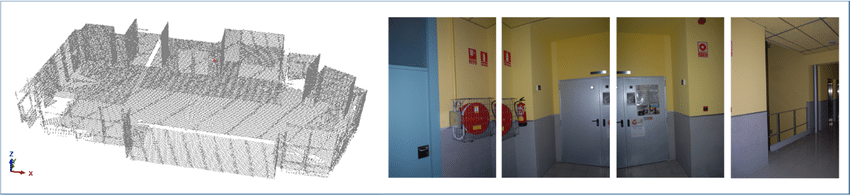
\includegraphics[width=0.9\linewidth]{images/point_cloud_and_images.png}
	\caption{The method data. This is useful to understand how information are acquired.}
\end{figure}

First of all, the point cloud is rotated in a way that the floor and ceiling are parallel to the x-y
plane and walls are parallel to either the x-axis or y-axis. Then, the point cloud is clustered to detect planar surfaces: horizontal regions are automatically classified into ``ceiling" and ``floor", while vertical
regions are submitted to a visual inspection for their identification and labeling. The wall surfaces are extracted from the point cloud and the corresponding RGB orthoimages are produced and aligned with them. The extraction of closed doors is carried out through an image-based algorithm applying the Generalized Hough Transform to the walls' orthoimages. This approach is invariant to scale changes and can handle reasonably small occlusions and noise. The first step consists on convert the wall images in grayscale, where edges are found by using the Canny operator. Then, using the Hough Transform, the candidate rectangles are detected using some constraints (like min and max width and height). This article is useful because explains how to generate the walls orthoimages. The point cloud and the corresponding images are captured at the same time and a ray-tracing algorithm selects the most suitable image sources to be aligned with the walls, avoiding wrong RGB projections and orthoimage areas without information.

\newpage

\section{RGB-D-Based Object Recognition Using
	Multimodal Convolutional Neural
	Networks: A Survey \cite{8683987}}

The work reported in \cite{8683987} is a survey of object recognition techniques that use both RGB and depth information collected synchronously. The authors highlight two key issues, namely, training data deficiency and multimodal fusion. The classical methods to recognize objects use only RGB data: they project the 3D world into a 2D space causing an inevitable data loss. Depth images can overcome this limitation. These types of data present many
advantages, being invariant to lighting and color variations, allowing better separation from the background, and providing pure geometry and shape cues. In recent years, deep learning methods, especially the CNNs, have become extremely popular to solve object recognition tasks. To improve their performance, discriminative features can be extracted independently from the RGB and depth data and then merged together, as shown in the figure below. This architecture is called MMCNN (Multi-Modal Convolutional Neural Network).

\begin{figure}[h!]
	\centering
	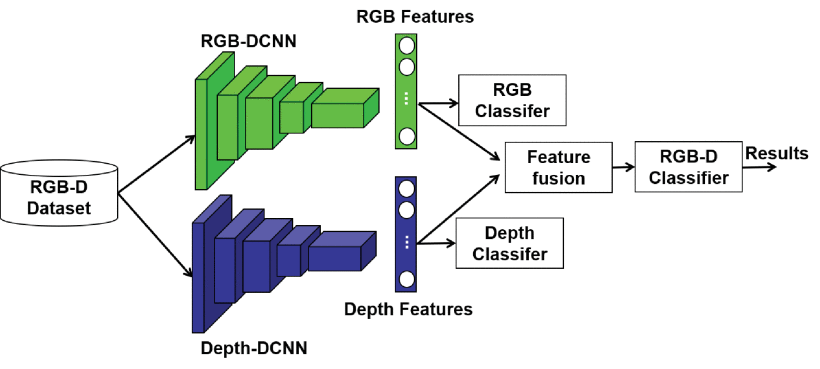
\includegraphics[width=0.8\linewidth]{images/cnn_rgb_depth.png}
	\caption{General framework of MMCNNs for RGB-D object recognition. This picture is useful to understand the general possible  architecture of a CNN which combines both RGB and depth data.}
\end{figure} 

In the MMCNNs based methods, training data deficiency and multimodal fusion are two key issues and challenges. First of all, RGB-D datasets, especially labeled data, are much more scarce compared to the RGB images. A possible solution  is to use an off-the-shelf CNN architecture pre-trained
on ImageNet and fine-tune it using the labeled RGB-D dataset, but depth data have a different color distribution. Furthermore, multimodal fusion is an active research topic in multimedia and this paper focuses on the RGB and depth modalities which can be considered as complete multimodal data. To do this, there are two main approaches: 

\begin{itemize}
	\item \textbf{Early fusion:} also known as \textbf{feature fusion}, integrates data from different modalities before being passed to a classifier. The RGB and depth features are extracted from two separate CNNs. Then the features from the two modalities are fused to meet the requirements for a deeper understanding of the captured information. The early level fusion is advantageous in that it can utilize the correlation between multiple features from different modalities at an early stage which helps in better task accomplishment.
	\item \textbf{Late fusion:} also known as \textbf{decision fusion}, integrates the responses obtained after individual features learning the model for each descriptor at the last stage. This method refers to the aggregation of decisions from multiple classifiers, each trained on separate modalities. This fusion architecture is favored because errors from multiple classifiers tend to be uncorrelated and it is feature independent.
\end{itemize}

A variety of methods have been proposed for RGB-D object representation and they can be mainly classified into three categories: hand-crafted feature-based methods, traditional feature learning-based methods, and MMCNNs based methods. We focus on the latter. In the supervised learning methods, an RGB-CNN and a Depth-CNN are constructed, or two off-the-shelf CNNs are fine-tuned based on the labeled RGB and depth data. Then, a multimodal fusion strategy is adopted to fuse the two modalities and finally, a classifier is trained for recognition.
The big problem with the supervised technique is the lack of large labeled datasets containing depth images. To avoid this fact, a semi-supervised method can be used. An RGB classifier and a depth classifier are trained to model the two modalities using a limited labeled training set (containing both RGB and depth data). Then, the trained classifiers are applied to
predict the examples from unlabeled training sets. The most confidently predicted instances of each class by
the two classifiers are transferred from unlabeled training set to labeled training set for the next round training.

\begin{figure}[h!]
	\centering
	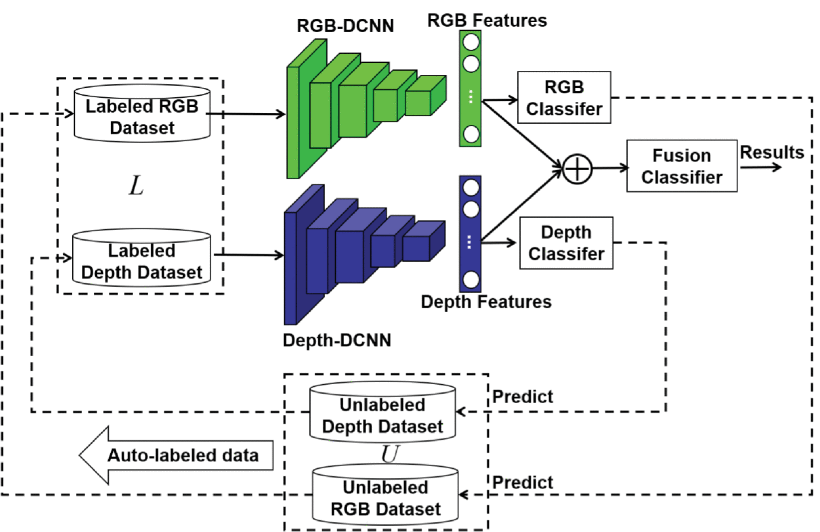
\includegraphics[width=0.8\linewidth]{images/cnn_semi_supervised.png}
	\caption{Overall structure of semi-supervised learning based MMCNNs
		for RGB-D object recognition.}
\end{figure} 

If a CNN has to elaborates depth data, they must be rendered in RGB images to emulate the distribution of the
corresponding RGB data. Many depth encoding methods were proposed which can be grouped into
two categories, namely, hand-crafted encoding methods and
learning-based encoding methods. The hand-crafted encoding methods are intuitive and easy to be implemented. Some of them are Surface normals, ColorJet, HHA, and Embedded depth. Since these methods are sub-optimal, in recent years a learning-based depth encoding method has been proposed. It uses a deep network to map the depth images to RGB images by exploiting a residual paradigm. Most of the state-of-the-art works in this domain adopted early
level fusion strategy because the features extracted from CNN are discriminative and easy to be fused. One technique in this domain is called \textbf{Fully-Connected Level Fusion}. Of the various ways of Fully-Connected Layer Fusion,
a straightforward approach is to use two different CNNs (one for RGB and another for depth data) and then chain together the final fully-connected layers of these two networks. This technique is called \textbf{Concatenated Fusion}.

\begin{figure}[h!]
	\centering
	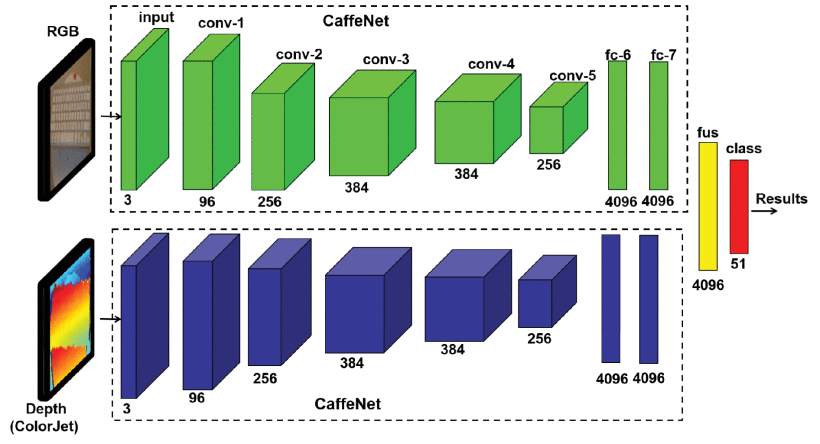
\includegraphics[width=0.8\linewidth]{images/cnn_merged_fcl.png}
	\caption{Concatenated fusion technique. The final fully-connected layers (called fc-7) are chained together in an end-to-end fashion. This image is useful to understand the Concatenated Fusion technique. }
\end{figure} 

The major issues of the technique explained above are that the relation between the two modalities is ignored
and the complementary nature of the modalities cannot be fully exploited. Also, it leads to very large input vectors that may contain redundancies. A possible solution is to fuse the fully-connected layer in a multimodal shared and modality-specific fashion. In \cite{75b99ea2e5664bf3842099e1f5f7ca63}, it is proposed a multimodal fusion layer that used matrix transformations to explicitly enforce a common part to be shared by features of different modalities while retaining modality-specific learning.

\begin{figure}[h!]
	\centering
	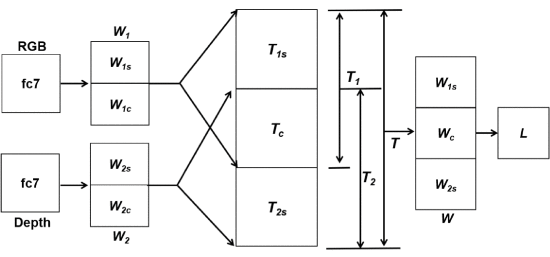
\includegraphics[width=0.6\linewidth]{images/fision_transofmration_matrix.png}
	\caption{The framework of matrix transformations for multimodal feature learning framework. $T_{1s}$ and $T2_s$ denote the RGB and depthmodal-specific parts, while $T_c$ is the common part. $T = [T_{1s}
		; T_c ; T_{2s}
		],
		W_1 = [W_{1s}
		; W_c ]$ and $W_2 = [W_{2s}		; W_c ]$ are the transformation matrix for
		RGB and depth modalities.  }
\end{figure} 

\newpage

To outperform these fusion methods, recent studies prove the advantages of the convolutional layers. This fact is used by Socher \textit{et al.} \cite{47876543}, that proposed a deep feature learning model
combing convolutional and recursive neural networks (CNNRNNs). The low-level features extracted by a single CNN layer are assembled by multiple RNNs and, finally, the RNN descriptors extracted from each modality were merged and fed to a joint softmax for classification.

\begin{figure}[h!]
	\centering
	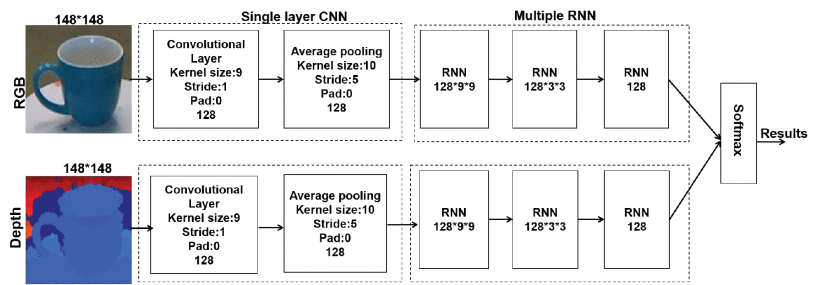
\includegraphics[width=0.6\linewidth]{images/CNNRNN.png}
	\caption{Overview of CNN-RNN model. This picture shows that it is possible to improve the performance of object recognition task using depth information.}
\end{figure} 


Another approach consists in to use the auto-encoders to learn low-level features from RGB and depth data. A recent strategy, reported in \cite{2342567}, the feature fusion (of RGB and depth data) took place in an earlier stage. In this work, a single CNN layer and average pooling strategy are utilized to learn low-level features from the RGB and depth modalities. Then the low-level features are fused in a united feature map and input to another CNN layer to extract high-level features. Last,
a kernel extreme learning machine (a feedforward neural network in which hidden nodes' parameters need not be tuned) is trained for classification. 

\begin{figure}[h!]
	\centering
	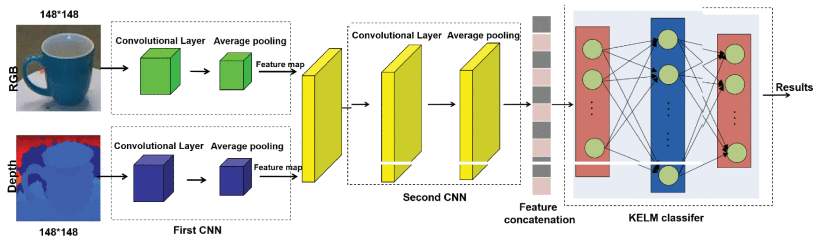
\includegraphics[width=0.8\linewidth]{images/cnn_early.png}
	\caption{The CNN-RNN model for RGB-D object recognition. This is useful to understand how to integrate features from both RGB and depth data after the early stage.}
\end{figure}

\newpage

In \cite{loghmani2019recurrent} volumetric features were extracted at different convolutional levels. At each level, the RGB-D features are linearized and then sequentially fed into a RNN concatenated in a unique sequential input. Last, the output of the RNN is used by the softmax classifier for the final prediction. Experimental results showed that the multi-level feature fusion method outperformed the single-level feature fusion method. 

\begin{figure}[h!]
	\centering
	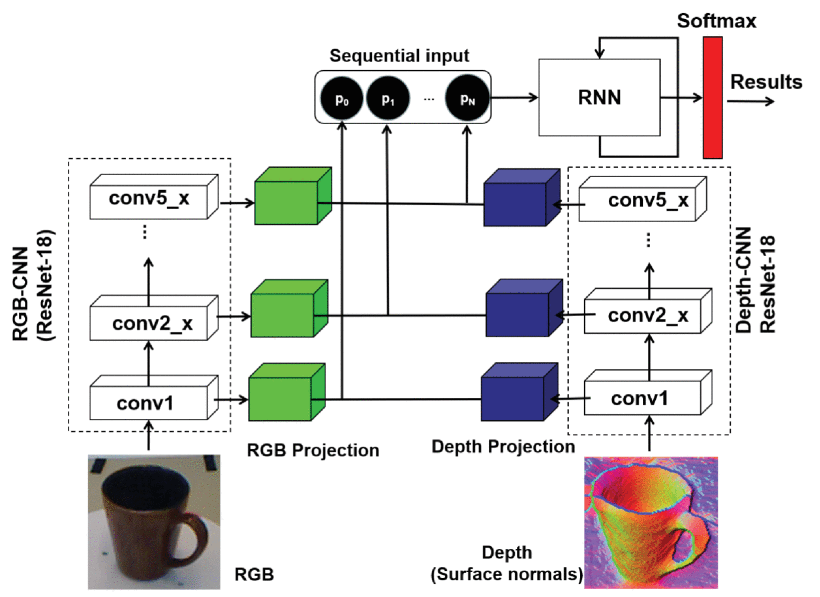
\includegraphics[width=0.8\linewidth]{images/sequential_fusion.png}
	\caption{Architecture of multi-level fusion method. This is picture shows how to fuse features extracted from different streams at different levels.}
\end{figure}

\newpage

Unlike early level fusion, the decisions (at the semantic level) usually have the same representation which enables the decision fusion much easier. The first late fusion method we examine is called Cascade Fusion. A pre-trained CNN extracts features for RGB, embedded depth, and embedded point cloud, respectively. After that, the hypercube pyramid features of convolutional layers and fully-connected layer features were first fed to two ELM (Extreme Learning Machines) classifiers to predict the class probabilities. Then, the concatenation of these new vectors was used as an input vector to another ELM for final classification.

\begin{figure}[h!]
	\centering
	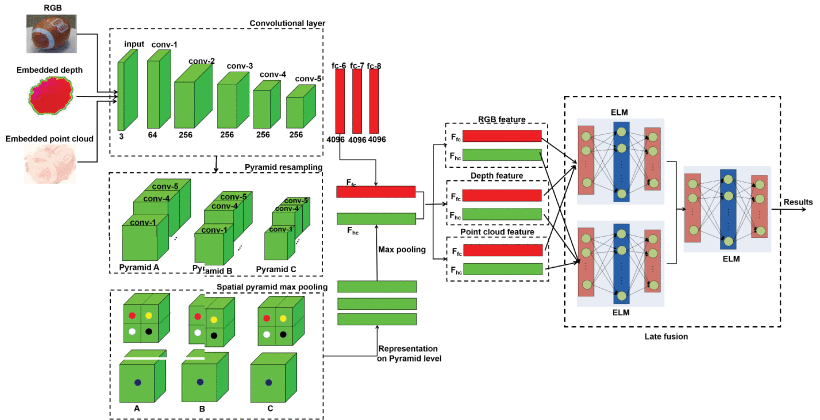
\includegraphics[width=0.8\linewidth]{images/late-fusion-elm.png}
	\caption{Overview of cascaded late fusion framework for RGB-D object recogniton. This picture is important because shows an easy fusion method. It outperforms the early fusion scheme which
		concatenated $F_{hc}$ and $F_{fc}$ simply.}
\end{figure}

In the hierarchical fusion technique, the class probabilities are determined by the fusion of class probabilities estimated at different hierarchical levels.  A typically hierarchical fusion 
for RGB-D object recognition was proposed by Asif \textit{et al.} \cite{8022892}. They divide the classification into image-level and pixel-level. The final object classification loss function
is a weighted combination of a pixel-level classification loss function and an image-level classification loss function.


Semi-supervised based methods address the problem of learning a better classifier by combining a small set of labeled data and a large amount of unlabeled data. These methods are also grouped into early level fusion
and late level fusion. The \textbf{Weighted Average Based Fusion} is the simplest but
the most commonly used late level fusion method in semi-supervised learning based MMCNNs for RGB-D object
recognition. This technique was first proposed in \cite{76543}. The authors utilize a CNN-RNN model to learn
features from RGB and depth modalities and train two
SVM classifiers from the labeled training sets. The two trained classifiers are applied to predict the examples from the unlabeled training sets. The most confidently
predicted instances of each class by the two classifiers are
transferred from unlabeled dataset to labeled dataset for the
next round of training. The algorithm runs until it reaches the
maximum number of iteration or the unlabeled pool is
empty. The category of the input instance is determined
by the weighted sum of the two probability scores generated
by the two classifiers.

\begin{figure}[h!]
	\centering
	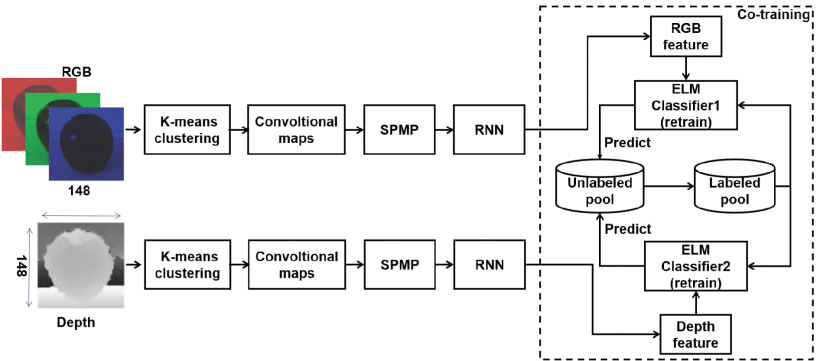
\includegraphics[width=0.7\linewidth]{images/cnn_rnn_semi_super.png}
	\caption{Co-training based semi-supervised learning for RGB-D object recognition. This method can be useful to use and include in training unlabeled data.}
\end{figure}

\newpage

The previous approach does not adopt deeper CNN architectures and early fusion schemes because the small labeled dataset is infeasible to supervise the training of a deep CNN model for object recognition. To overcome this barrier, Cheng \textit{et al.} \cite{cheng2016semi-supervised} utilize two reconstruction networks to decode each channel of the inputs using both the labeled and unlabeled data. When the reconstruction network of each modality
achieve convergence, the parameters of the convolutional
layers were utilized to initialize the corresponding convolutional layers of each modality in the proposed configuration. Then a diversity preserving co-training algorithm is implemented to select highly confident examples with predicted labels from the unlabeled pool. Last, a fusion classification layer was added by concatenating the two end-layers and the entire model was optimized end-to-end. 

\begin{figure}[h!]
	\centering
	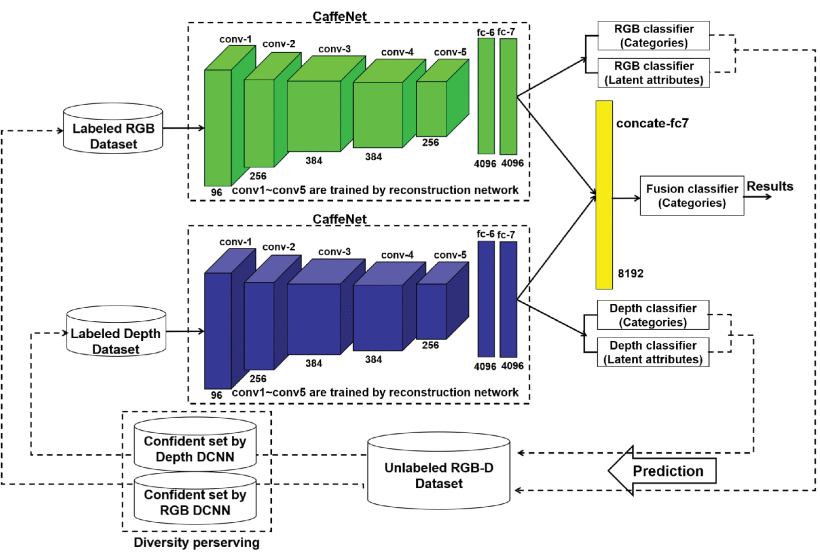
\includegraphics[width=0.7\linewidth]{images/semi_super_all.png}
	\caption{Overall framework of diversity preserving co-training method. This image is useful to understand a possible approach in which the two CNNs are initialized using both labeled and unlabeled data.}
\end{figure}

This survey is really important because summarizes the most relevant object recognition works based on deep learning techniques, that use both RGB and depth data. In addition, a detailed report of the existent dataset is included in the second part of the article. 


\newpage

\section{Automatic Room Segmentation From Unstructured 3-D Data of Indoor Environments \cite{7814251}}

In \cite{7814251} the authors propose an automatic approach for the task of
reconstructing a 2-D floor plan from unstructured point clouds
of building interiors, without prior knowledge. In addition, this work provides an accurate algorithm to recognize walls and openings. 

\begin{figure}[h!]
	\centering
	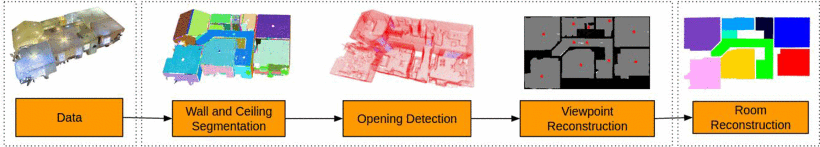
\includegraphics[width=0.9\linewidth]{images/segm_method.png}
	\caption{Method overview. This figure explains in detail the steps that make up the paper's algorithm.}
\end{figure}

First of all, the method captures the floor point cloud and segments it to detect walls and ceilings. Then, the proposed approach proceeds to search for openings, defining them as any portion of empty space contained within planar wall segments which is the required size and shape. The next step is called \textit{Viewpoint Generation}: in this phase, the point cloud are projected in a 2D image and, using this, the viewpoints are found. A viewpoint is a pixel in the image that observes the major part of the pixels in the free space around itself. Finally, the proposed method performs the \textit{Room Reconstruction} phase. The 3D points of the environment's point cloud are labeled according to the viewpoint they can see. Next, an initial room segmentation is performed and it is subsequently refined merging regions belonging to the same room.

\begin{figure}[h!]
	\centering
	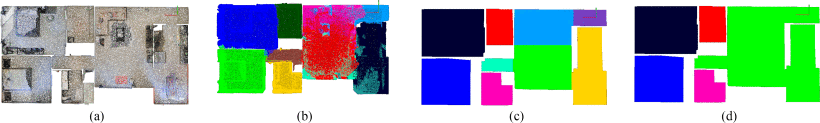
\includegraphics[width=0.9\linewidth]{images/room_seg.png}
	\caption{Room reconstruction end-to-end: (a) Initial point cloud. (b) Initial viewpoint labeling of point cloud - each color represents points associated with a
		different viewpoint. (c) Initial room segmentation. (d) Final room segmentation, after merging. This figure is useful because it explains how to perform room segmentation starting from a 3D point cloud, applying the information obtained from the previous steps.}
\end{figure}

This work introduces a method to segment a space in rooms, so finding the rooms' connections can give a possible location where to find a potential room. 

\newpage

\section{Semantic Labeling of Indoor Environments from 3D RGB Maps \cite{8462922}}
The work in \cite{8462922} is based on \cite{7814251}. It presents an approach to automatically assign semantic labels to rooms reconstructed from 3D RGB maps of apartments. The proposed method uses deep-learning techniques for scene classification and object detection. The method input is a mesh representation of the environment. First off all, the authors generate a 2D segmentation as presented in \cite{7814251}. Then realistic-looking images are rendered to be used in the following classification steps ( the authors do not have access to the original data used to create the environment mesh). At each viewpoint 36 partly overlapping images are rendered with a horizontal rotational step size of 10 degrees to cover 360 degrees. These images are used by a CNN to perform two different classifications: Scene Level and Object Level. 

\begin{figure}[h!]
	\centering
	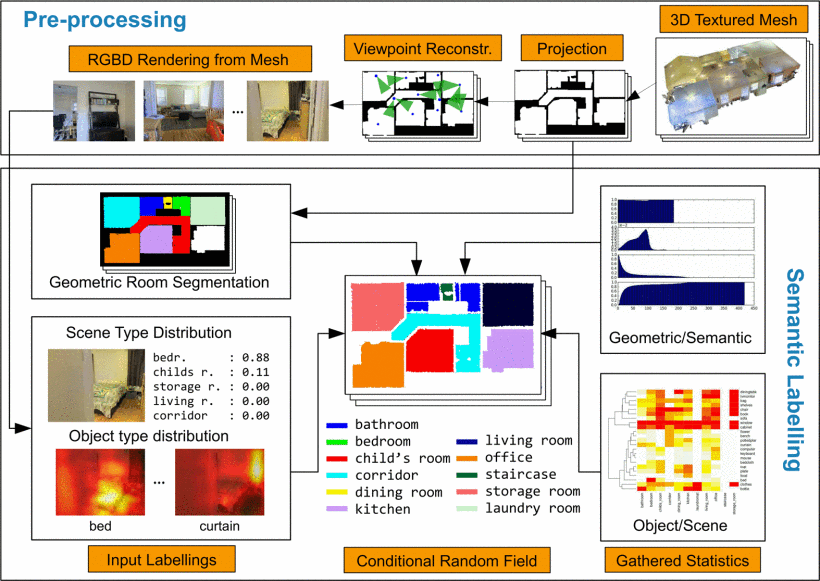
\includegraphics[width=0.9\linewidth]{images/semantic_label_overview.png}
	\caption{Overview of the proposed system for semantic room tagging. This can be useful to understand how the method works and what are the steps to prepare the data that will be processed by the classification module.}
\end{figure}

The use of these information can split further the initial 2D room segmentation. The proposed method performs a Scene Level classification, in which a neural network is trained on a select pool of images taken from Place 365. Despite the good results obtained, many scenes are ambiguous or are difficult to label. To refine this process, the authors performs also a Object Level Detection. In fact, certain objects are highly indicative of the scene type, and detect them in a scene can help to successfully label it.

\begin{figure}[h!]
	\centering
	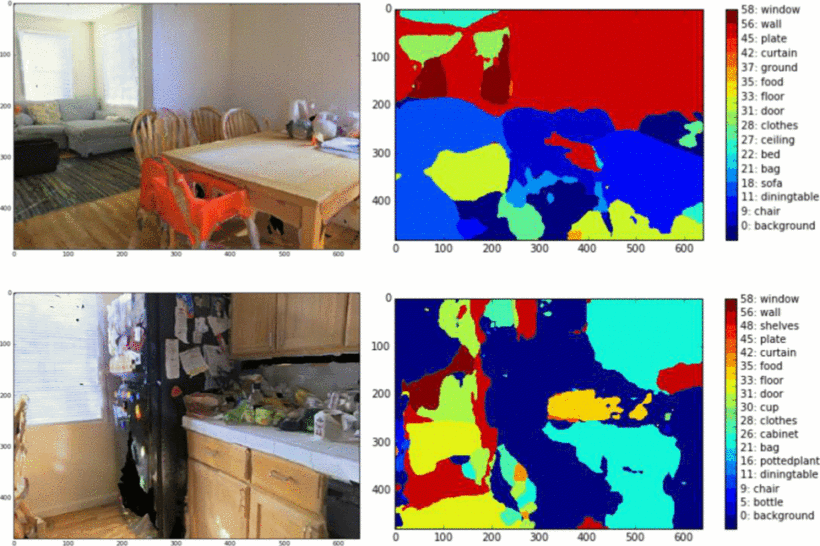
\includegraphics[width=0.7\linewidth]{images/object_dete.png}
	\caption{Results of the object detection module. This image visually explains the output of the object classification module.}
\end{figure}

Next, it is necessary to learn a model for which links object detection to the appropriate room types.

\begin{figure}[h!]
	\centering
	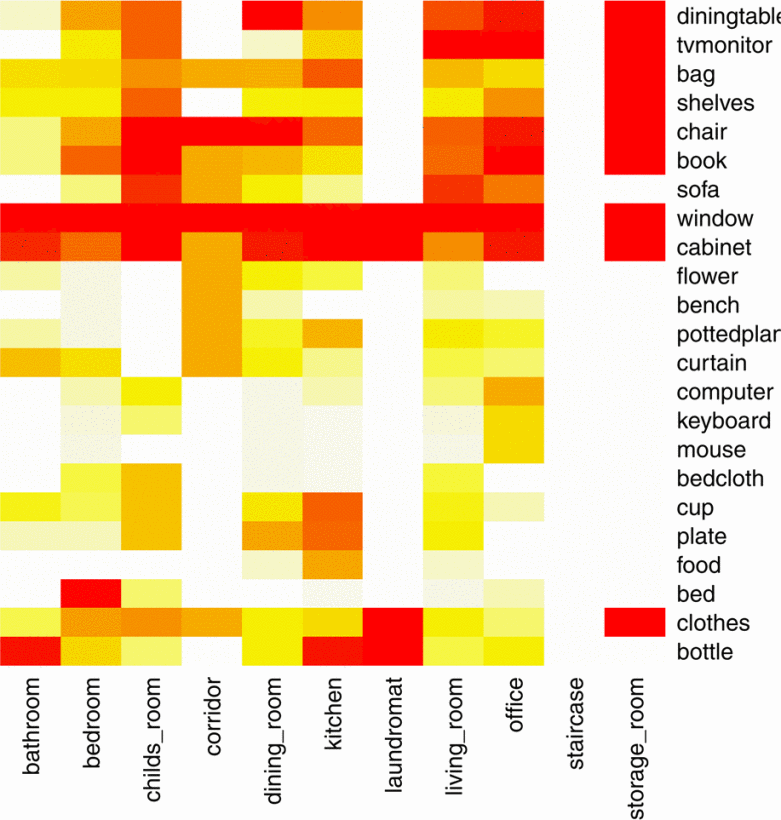
\includegraphics[width=0.5\linewidth]{images/obkject_in_rooms.png}
	\caption{Occurrence frequencies of the most important object categories in scene types. This picture is useful to understand what is he relations between objects and room types.}
\end{figure}

\newpage

Finally, the proposed method merges the different cues to generate a more accurate and robust final scene classification. Each pixel, of the 2D segmentation, is modeled as a set of random
variables consisting of the corresponding probability distributions of the scene class labeling and the
object. This method explains clearly how to use the information obtained before to assign a label to each pixel. This work is useful to understand how semantic labeling an environment mainly using data obtained with deep models and how to aggregate them. Also, this article analyses different image datasets and selects the best for this purpose.  

\newpage

\section{From Pixels to Buildings: End-to-end Probabilistic Deep Networks for
	Large-scale Semantic Mapping \cite{8967568}}

In \cite{8967568} the authors present TopoNets: end-to-end probabilistic deep networks for modeling semantic maps. The proposed method is based on the Sum-Product Network, a probabilistic model that combined with deep learning can acquire hierarchical probabilistic models directly from high-dimensional and noisy data.

\begin{figure}[h!]
	\centering
	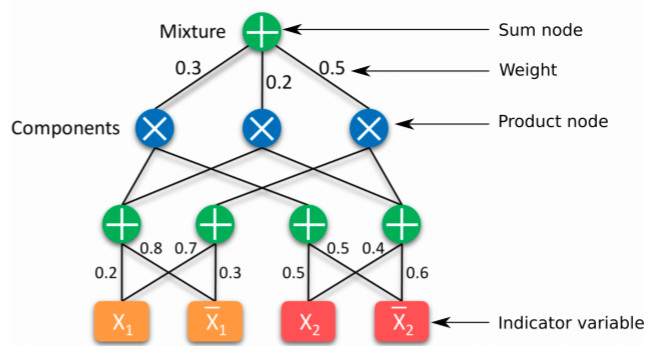
\includegraphics[width=0.7\linewidth]{images/SPN.jpg}
	\caption{An example of SPN. This picture explains clearly the architecture of an SPN. The bottom layer consists of indicators for different values of the variables X1 and X2, that belong to different domains.}
\end{figure}

In this work, the authors use a simple structure learning technique which begins by initializing the SPN with a random dense structure that is later pruned. A semantic map is defined as a growing topological graph of places associated with observations of local geometry as well as semantic descriptions. The nodes in this graph represent places the robot can visit and the edges represent both navigability and spatial relations. Each place is associated with its local geometry representations and latent variables representing semantics. More formally, the authors specify a semantic map as $ M = (T, X, Y)$, where $T = (V,E)$ is a topological graph with vertices $V$ and
edges $E$, and $X = \{X_i : i \in V \}$, $Y = \{Y_i : i \in V \}$. A set of sub-maps templates can be used to decompose a semantic map ($X_i$ denotes local observations of a place
geometry while and $Y_i$ is the semantic attributes that describe that place). During the Learning Phase, a robot incrementally constructs a topological graph and obtain local sensory observations at each place. These local observations are transformed into a robot-centric polar
occupancy grid. The authors define a set of sub-map templates: their structure and parameters are learned using the dataset of matching map parts. Next, when a robot has to inference the topological map of an environment, it constructs a topological graph. Then, a trained TopoNet is adapted to the topological structure of the underlying semantic map $M_{test}(T,X,Y )$ and latent
place semantics is inferred.

\begin{figure}[h!]
	\centering
	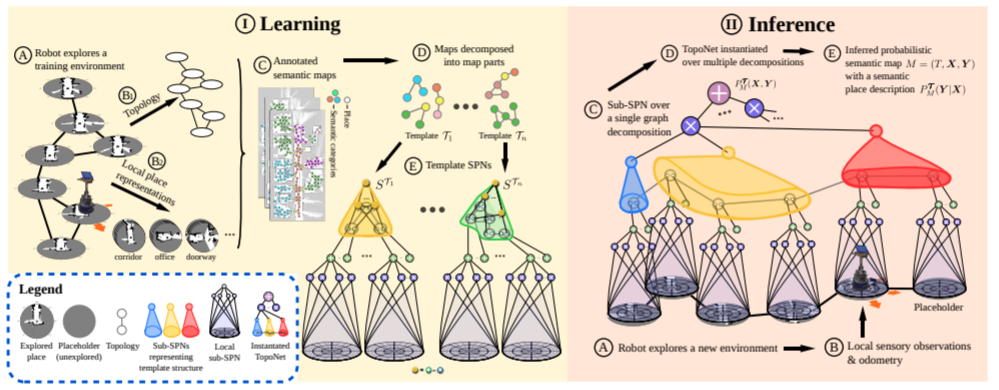
\includegraphics[width=0.8\linewidth]{images/SPN_training_inference.png}
	\caption{Learning and inference process with TopoNets. This is useful to understand how TopoNet operates.}
\end{figure}

\newpage

This work is particularly useful because it solves the problems of door detection in a different way: it models a doorway as a connection of two different semantic places, with a dedicated node in the semantic map. A doorway can be a plausible location of a physical door.

\begin{figure}[h!]
	\centering
	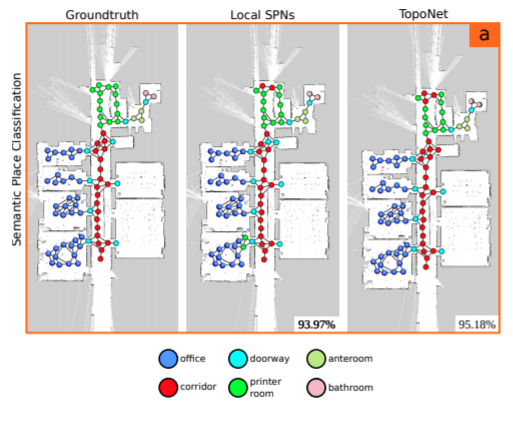
\includegraphics[width=0.8\linewidth]{images/SPN_example.png}
	\caption{An example of Toponet inference. This image shows that TopoNet identify doorways.}
\end{figure}

\section{YOLOv3: An Incremental Improvement \cite{yolov3}}

This paper presents the YOLO v3 architecture. YOLO is a neural network that performs object detection inside images. Classical approaches consist of using classifiers or localizers to perform detection. These methods apply the model to an image at multiple locations and scales and the high-scoring regions of it ar considered detections. YOLO uses a totally different approach. It applies a single neural network to the full image. This network divides the images into regions and predicts bounding boxes and probabilities for each region. This model has some advantages. First of all, the whole image is considered, so the global context influences the prediction. Next, YOLO is extremely fast because it uses a single network, differently from other methods (like R-CNN) that uses thousands of them. The third version of YOLO is characterized by some design changes, that make it a little bigger than the previous version, but still faster. YOLO v3  predicts \textbf{bounding boxes} using dimension clusters as anchor boxes. The
network predicts 4 coordinates for each bounding box, $t_x$,
$t_y$, $t_w$, $t_h$. More precisely, if the cell is offset from the top left corner of the
image by $(c_x, c_y)$ and the bounding box prior has width and
height $p_w$, $p_h$, then the predictions correspond to: 
\begin{align*}
&b_x = \alpha(t_x) + c_x \nonumber \\
&b_y = \alpha(t_y) + c_y \nonumber \\ 
&b_w = p_w e^{t_w} \nonumber \\  
&b_h = p_he^{t_h} \nonumber 
\end{align*}

\begin{figure}[h!]
	\centering
	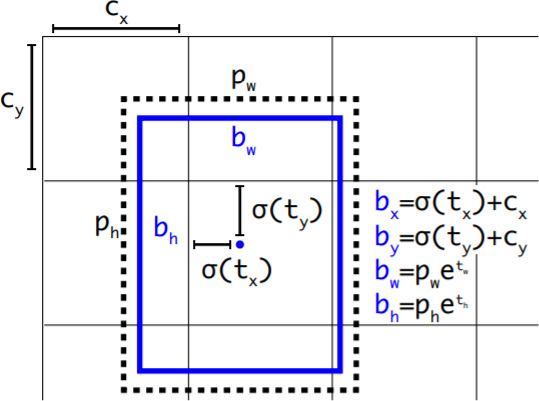
\includegraphics[width=0.5\linewidth]{images/bound.png}
	\caption{This picture is useful to understand the YOLO's prediction. It predicts the width and height of the box as offsets from the cluster centroid.}
\end{figure}

During training, YOLO v3 uses sum of squared error loss. If the
ground truth for some coordinate prediction is $\hat{t}_*$, the gradient is the ground truth value (computed from the ground
truth box) minus our prediction: $\hat{t}_* - t_*$. This ground truth
value can be easily computed by inverting the equations
above.
\newpage 

The \textbf{class prediction} is based on the bounding boxes: e label is assigned to each of them. During training, the binary cross-entropy loss for the class
predictions is used. YOLO v3 is also able to make \textbf{predictions across different scales}. In particular, it predicts boxes at 3 different scales. YOLO v3 extracts features from those scales using a similar concept to feature pyramid networks \cite{DBLP:journals/corr/LinDGHHB16}. A network that performs object recognition must be able to detect the same object at different scales. The standard solution consists into learn feature pyramids through image pyramids (Fig. \ref{fig:pyramids}(a)). An image pyramid is a sequence of the same image at different scales. The features are computed on each of the image scales independently: this is extremely slow. This method has been replaced with the convolutional networks, which produce a single feature map that are more robust to scale variance and thus facilitate recognition from features computed on a single input scale (Fig. \ref{fig:pyramids}(b)). An extension of this method is to featuring each level of the image pyramid, producing a multi-scale feature representation in which all levels are semantically strong. Nevertheless, featurizing each level of an image pyramid has obvious limitations. Inference time increases considerably. In addition, training end-to-end networks on image pyramids is infeasible in term of memory.
However, image pyramids are not the only way to compute a multi-scale feature representation. A deep convolutional neural network computes a feature hierarchy layer by layer, and with subsampling layers the feature hierarchy has an inherent multiscale, pyramidal shape. This feature hierarchy
produces feature maps of different spatial resolutions, but
introduces large semantic gaps caused by different depths. One of the first attempts at using this approach is called SSD: Single Shot Detector (Fig. \ref{fig:pyramids}(c)).
This approach would reuse the multi-scale feature
maps from different layers computed in the forward pass
and thus come free of cost. But to avoid using low-level
features SSD foregoes reusing already computed layers and
instead builds the pyramid starting from high up in the network and then by adding
several new layers. Thus it misses the opportunity to reuse
the higher-resolution maps of the feature hierarchy, which are important for detecting small objects.
The method proposed in \cite{DBLP:journals/corr/LinDGHHB16} is to improve the method explained above, creating a feature pyramid with a strong semantic at all scales. To achieve this goal, the authors rely on an architecture that
combines low-resolution, semantically strong features with
high-resolution, semantically weak features via a top-down
pathway and lateral connections (Fig. \ref{fig:pyramids}(d)). This result is obtained quickly using only a single image as input.

\begin{figure}[h!]
	\centering
	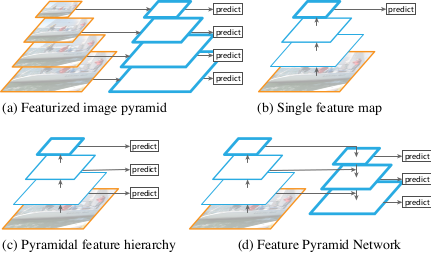
\includegraphics[width=0.5\linewidth]{images/pyramid.png}
	\caption{This figure gives a visual representation of the previous methods to collect scale independent features. (d) The method proposed by this work.}
	\label{fig:pyramids}
\end{figure}


This approach takes a single-scale image of an arbitrary size as input, and outputs proportionally sized feature maps at multiple levels, in a fully convolutional fashion. The construction of the pyramid involves a bottom-up pathway, a top-down pathway, and lateral connections. The \textbf{bottom-up pathway} is the feedforward computation of the convolutional network, which computes a feature hierarchy consisting of feature maps at several scales with a scaling step of 2. There are often many layers producing output maps of the same size and we say
these layers are in the same network \textit{stage}. The authors define a \textit{pyramid level} for each \textit{network stage}. The \textbf{top-down pathway} hallucinates higher resolution features by
upsampling spatially coarser, but semantically stronger, feature maps from higher pyramid levels. These features are
then enhanced with features from the bottom-up pathway
via lateral connections. Each lateral connection merges feature maps of the same spatial size from the bottom-up and the top-down pathways. 
The Fig. \ref{fig:topdownpath} shows the building block that constructs our top-down feature maps. A coarser-resolution feature map is upsampled by a factor of 2 (using a nearest neighbor upsampling for simplicity). This upsampled map is then merged with the corresponding bottom-up map by element-wise addiction.

\begin{figure}[h!]
	\centering
	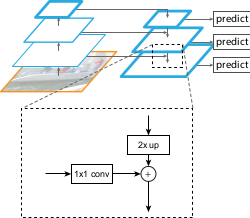
\includegraphics[width=0.5\linewidth]{images/topdownpath.png}
	\caption{A building block illustrating the lateral connection and
		the top-down pathway, merged by addition. This figure is useful to understand how the top-down path is built.}
	\label{fig:topdownpath}
\end{figure}

The feature extractor used in YOLO v3 uses a similar concept to feature pyramid networks, but several convolutional layers are added to the base classical pyramid network architecture. The last layer predicts a 3d tensor encoding bounding box, objectness and class predictions. For example, if 3 boxes are predicted at each scale, the tensor could be $ N \times N \times [3 \ast (4 + 1 + 80)] $, where 4 are the bounding box offsets, the objectness is 1 and the class predictions are 80. 
To perform feature extraction, the authors use a new approach. This network implies successive $3 \times 3$ and $1 \times 1 $
convolutional layers but now has some shortcut connections and it is significantly larger. It has 53 convolutional layers.

\newpage 

\section{Improving Repeatability of Experiments
	by Automatic Evaluation of SLAM Algorithms \cite{8594189}}

In this paper, the authors propose an approach to improve the repeatability of experiments performed in robotics. In particular, they focus on the domain of SLAM (Simultaneous Localization And Mapping). In this work, it is introduced a system that exploits simulations to generate
a large number of test data on which SLAM algorithms are
automatically evaluated in order to obtain consistent results,
according to the principle of repeatability. \textit{Reproducibility} is the possibility to verify, in an independent
way, the results of an experiment. This means that other experiments should achieve the same results when starting from the initial conditions, using the same
type of instruments and parameters, and adopting the same
experimental techniques. On the other hand, following the \textit{Repeatability} principle, a single result is not sufficient to ensure the success of an experiment.  A successful experiment must involve a large number of different trials, in order to guarantee that the results are not been achieved by chance, but to ensure that they are systematic. In the robotics domain, the SLAM algorithms present some variability when they are used to collect data in the same environment with different runs. This fact is shown in this work. The authors present a simulation system to generate a large number of test data on which SLAM algorithms are automatically evaluated to obtain consistent results according to the principle of repeatability. Finally, this system is validated showing that the performance of a SLAM algorithm applied to test data is very similar to the performance of the same algorithm applied to data comes a real robot.
In general, running experiments for testing SLAM algorithms involves three main elements: the algorithm, the test
data, and the metric. The \textit{algorithm} we consider in this paper
is GMapping.  The test data are generated by the authors using simulation. This is because the existing datasets are obtained performing a single run per environment. The metric and the automatic way to apply it are exposed afterward. The evaluate the performance of GMapping, the authors consider a set of 100 indoor environments $\varepsilon$, with different sizes and shapes. Each environment $E\in \varepsilon$ is represented as a png image, with a resolution of $0.05 \times 0.05$ meters per grid cell (pixel). For each environment $E \in \varepsilon$, a set of test data $D_E$ is collected to be fed to GMapping. Each exploration run $R_E$ considers an environment $E$ and a starting position. The robot autonomously navigates in the partially unknown environment using the frontier exploration approach exposed in \cite{613851}. Each run ends when two consecutive snapshots of the grid map produced by GMapping are similar enough. The data collected in each run $D(R_E)$ included the laser range scans and odometry readings collected along the path followed to cover environment $E$. These data
are fed to GMapping which, at the end of the exploration,
produces the grid map $M(R_E)$. This process is iterated until a certain number of runs $|R_E|$ is performed for each environment. The metric used by the authors to assess the performance of SLAM algorithm is a variant of the \textit{localization error} metric, which measures the ability of SLAM algorithms to measure the actual trajectory followed by the robot. 

\begin{figure}[h!]
	\centering
	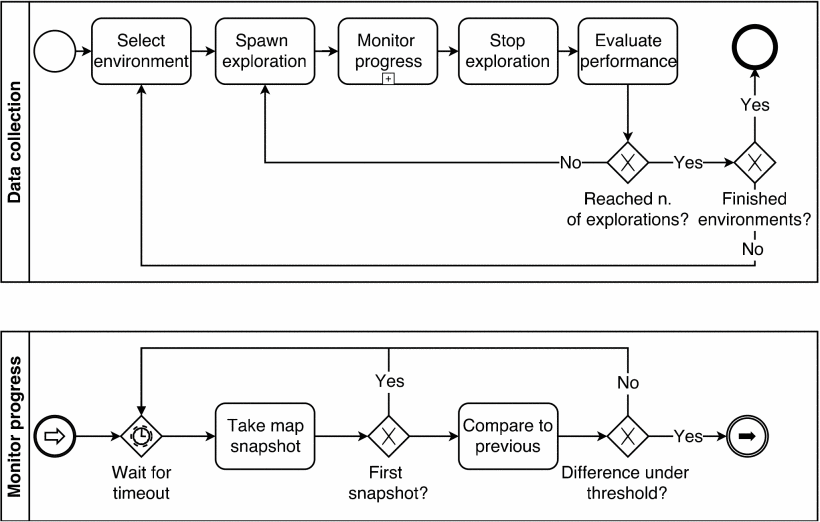
\includegraphics[width=0.7\linewidth]{images/explore_sequence.png}
	\caption{This figure shows the workflow of the systems proposed in this work.}
	\label{fig:explore_sequence}
\end{figure}

\newpage

\section{Place Categorization and Semantic Mapping on a Mobile Robot \cite{7487796}}

This paper focuses on the problem of place categorization and semantic mapping without environment-specific training.  Prior domain knowledge is incorporated by embedding the classification system into a Bayesian
filter framework that also ensures temporal coherence. The authors show that semantic information can boost robotic object detection performance and the semantic map can be used to modulate the robot's behavior during the navigation task.
The problem to assign a semantic label to places or environment's parts is often called \textit{place categorization} or \textit{semantic mapping}. To address this challenge the authors  focus on \textit{transferable} and \textit{expandable} semantic place categorization and mapping for robotics, combining vision and laser range data. \textit{Transferable} means the categorization does not require environment-specific training. To ensure this property, the convolutional neural networks specifically trained for place categorization are used in this work. These networks are able to generalize well and they do not have to be re-trained for specific environments. However, the ConvNet can recognize only the classes they have been trained on. The authors overcome the \textit{closed-set} condition and present a novel \textit{expandable} classification system by implementing ConvNet with a one-vs-all classifier that is able to recognize new classes online and is cheaper to train. In a typical computer vision application, each image is treated individually, but in a robotic system, robots see a temporal coherent stream of frames. This fact allows the authors to embed the semantic classifier in a Bayesian filter framework, to obtain more coherent results and  incorporate prior knowledge.

\newpage

The proposed place categorization system consists of four parts:
\begin{enumerate}
\item a convolutional neural network that classifies each image individually,
\item one-vs-all classifiers that recognize scene classes the
network was not trained on,
\item a Bayesian filter to exploit temporal coherence and
remove spurious false classifications, and
\item the mapping subsystem that gradually builds a map
using the resulting place labels.
\end{enumerate}

To classify each image individually, the authors use the Place205 network published in \cite{alma991017170972206031}. This network is trained specifically for the task of place categorization, the dataset comprised 2.5 million images of 205 semantic categories. The network input are RGB images, while its output are the probabilities over the 205 known classes. A possible way to overcome the closed-set condition of the Place205 classifier, is to retrain the entire network. This approach is computationally expensive (typical training times are in the order of days). To solve this issue, the authors propose an alternative method: a Random Forest one-vs-all classifier is trained using only a few (in the order of 10-100) training images. This classifier use the output of the fc7
layer of the Places205 network as a feature vector, which is the last generic fully connected layer. To incorporate the temporal dimension in the classification module, the authors use a Bayesian filtering technique. Interpreting place categorization as a Bayesian estimation problem allows the authors to incorporate other sources of
information in a very natural way. For instance, there are some places in the 205 categories defined by place Places205 that are unlikely or even impossible to be observed in a specific environment type. This information can be easily incorporated into the Bayesian filter's formula. The output of the Bayesian filter is the input of the semantic mapping component. In particular, this module produces a semantic and metric map of the environment, producing a grid map with a semantic layer for each semantic category. Fig. \ref{fig:grid_semantic_map} exposes this concept.

\begin{figure}[h!]
	\centering
	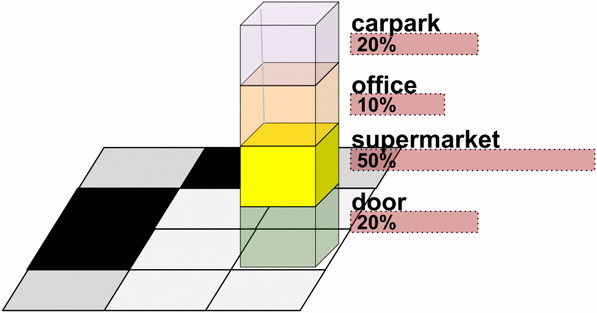
\includegraphics[width=0.7\linewidth]{images/gird_map_semantic.png}
	\caption{An illustration fo the semantic map structure. Level zero is the occupancy grid, while the higher levels encode encode the probabilities that a grid cell belongs to a
		certain semantic category. This picture explains clearly how the grid semantic map is built.}
	\label{fig:grid_semantic_map}
\end{figure}

\newpage

The result map is obtained propagating the class probability along the laser rays that are within the field of view of the
camera and updating the penetrated map cells using the usual
recursive Bayes filter update method \cite{246776423} for occupancy
maps. This method is able to correct spurious false classifications, since the probabilities inside cells are adapted and corrected with later observations. This article shows how to embed a deep learning classifier in a Bayesian filter, in order to enforce temporal coherence of the classification results. Another interesting this work introduces is a technique to overcome the closed-set condition, typical of the classical deep techniques. Despite this, a small retrain process has to be done to add new classes to the classifier that performs place categorization.

\section{The ThreeDWorld Transport Challenge: A Visually Guided
	Task-and-Motion Planning Benchmark for Physically Realistic Embodied AI \cite{gan2021threedworld}}

The authors introduce a visually-guided and physics-driven taskand-motion planning benchmark, which they call the ThreeDWorld Transport Challenge. In this challenge, an autonomous agent equipped with two articulated arms, find a small set of objects scattered in the environment, puck them up, and transport them in a desired location. This agent operates in simulated worlds. In addition, the authors position various containers in the environment: in this way the agent can collect some object in a single container and then transport multiple objects at the same time, as shown in Fig. \ref{fig:method}.

\begin{figure}[h!]
	\centering
	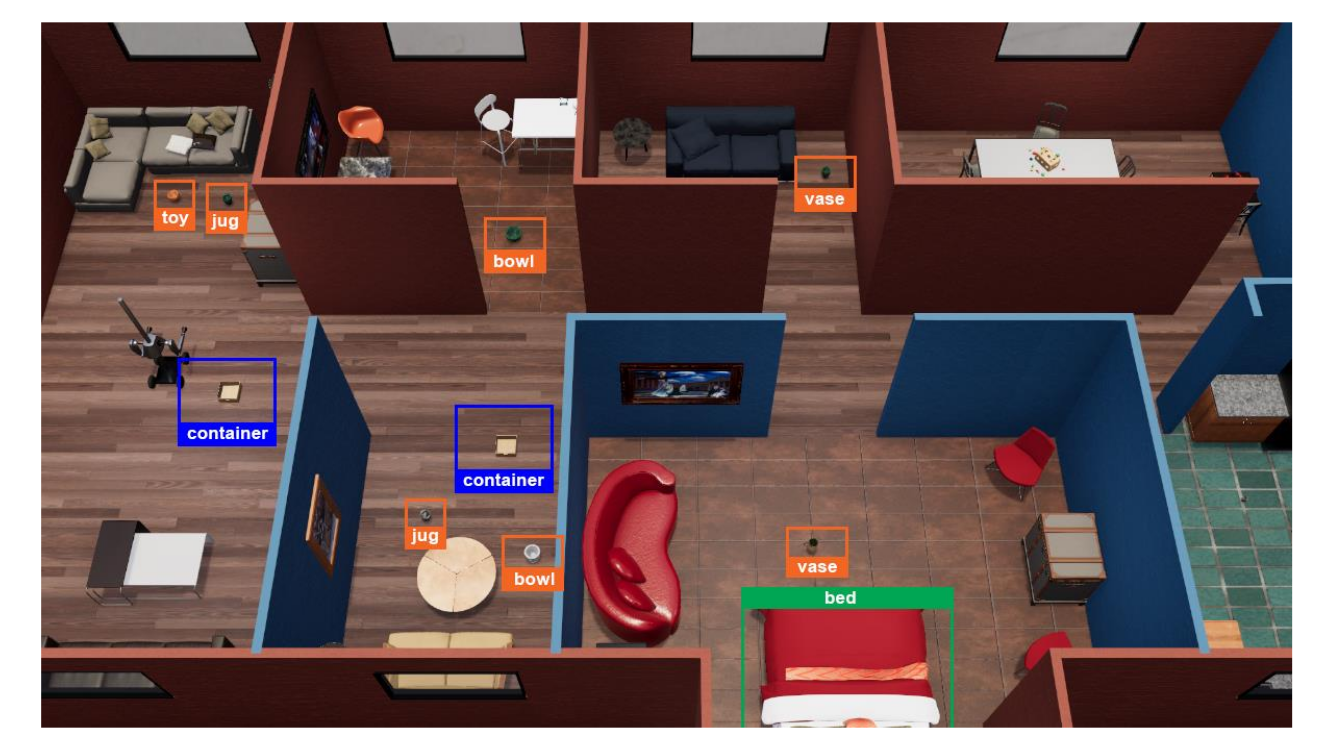
\includegraphics[width=0.7\linewidth]{images/challenge_move_object.png}
	\caption{This figure shows an example task. The agent must transport objects
		scattered across multiple rooms and place them on the bed (marked with a green bounding box) in the bedroom. To optimize it, the robot use a container to transport multiple objects.}
	\label{fig:method}
\end{figure} 

\newpage
This task is performed in physical realistic worlds, so it poses several challenges beyond semantic exploration of unknown environment, including:

\begin{itemize}
\item \textbf{Synergy between navigation and interaction.} The
agent cannot move to grasp an object if this object is
not in the egocentric view, or if the direct path to it is
obstructed (e.g. by a table).
\item \textbf{Physics-aware Interaction.} Grasping might fail if the
agent’s arm cannot reach an object.
\item \textbf{Physics-aware navigation.} Collision with obstacles
might cause objects to be dropped and significantly impede the transport efficiency.
\item \textbf{Reasoning about tool usage.} While the containers
help the agent transport more than two items, it also
takes some time to find them. The agent thus has to
reason about a case-by-case optimal plan.
\end{itemize}

As shown in Fig. \ref{fig:transport_challenge}, an embodied agent is required
to transport a set of predefined objects to a target location.
There are three types of objects that the agent needs to pay
attention to:
\begin{itemize}
\item Target objects: objects the agent needs to grasp and
transport, placed at various locations in the house.
\item Containers: objects that can be used as tools to assist with the transport of target objects, also located in
various rooms.
\item Goal position: a goal area is defined around one
unique object (e.g, a bed) in the house.
\end{itemize}

\begin{figure}[h!]
	\centering
	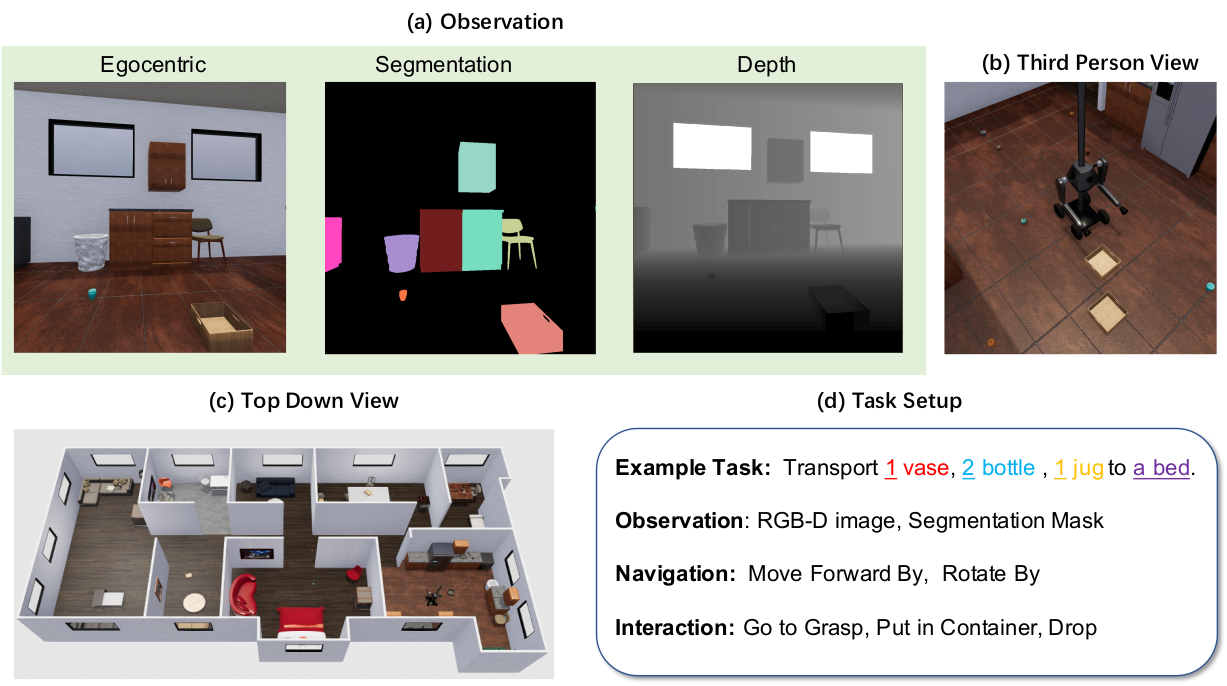
\includegraphics[width=0.8\linewidth]{images/transport_challenge.png}
	\caption{This figure is useful to understand the challenge reported in this work.}
	\label{fig:transport_challenge}
\end{figure}

Since that the object list and the goal location are varied in each task instance, the robot has to learn how explore an environment to find the objects and locations of interest. After that, the robot can plan a series of actions to complete the assigned task, 
always paying attention to respect the physics constraints. The authors created a series of 15 environment with 6-8 rooms, furniture and other items. The embodied agent used in the challenge is Magnebot. It is equipped with a RGB-D camera and two articulated arms to interact with the environment. The experimental setup is organized as follow. 10 environments are used as training set, while the remaining 5 as test set. The authors generate 100 tasks for each the seen houses (training set) and 20 tasks for each unseen house by randomly
placing target objects and containers into different rooms. The objective of this challenge is to
transport the maximum number of objects as efficiently as
possible. They use the transport rate as an evaluation metric.
The transport rate is the fraction of the objects successfully
transported to the desired position within a given interaction
budget (defined as a maximum episode length in steps). For
testing, the maximum episode length is set to 1000 steps.
To evaluate this challenge, the authors implemented several baseline agents using both
learning- and planning-based algorithms, but they found empirically that it was difficult for an end-to-end RL learning model solve efficiently this difficult task. Therefore, they
implemented additional baselines using a hierarchical planning framework with different exploration strategies. The authors define four types of sub-goals
for this task: \textit{exploration}, \textit{pick up a container}, \textit{pick up an
object}, and \textbf{place}. They use a rule-based high-level planner to
decide when to transition between sub-goals. For the exploration sub-goal, the agent will either directly use the policy
to navigate around the environment (RL Exploration baseline) or plan a shortest path from the current location to the
waypoints (Active, Frontier and Semantic Exploration baselines). The folloqing figure reports the baselines just explained. 

\begin{figure}[h!]
	\centering
	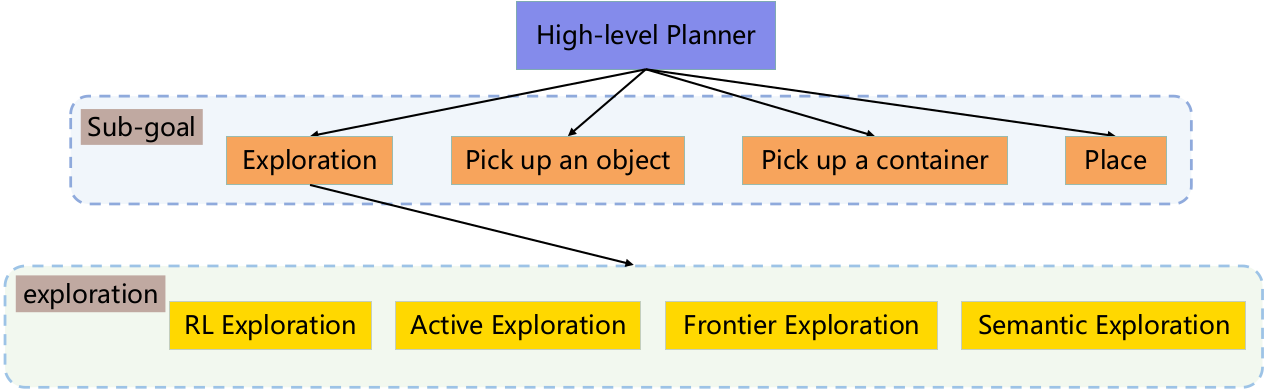
\includegraphics[width=0.9\linewidth]{images/baselines.png}
	\caption{The flowchart of high-level and low-level planners.}
\end{figure} 